\chapter{Descriptive Part}
\newpage
\section{Domain Description}
\subsection{Domain Rough Sketch}
Our application domain of interest is the \textbf{sneaker head} market domain. In this domain there are \textbf{secondhand sellers} who sell \textbf{limited edition shoes} to \textbf{customers}. Currently in Puerto Rico there is no platform that specializes in the \textbf{reselling} of \textbf{sneaker head} shoes with the \textbf{guarantee} that they are \textbf{legitimate}. From our initial meetings it was found that the second hand shoe market is a booming market with projected year over year growth. With this in mind we further set on finding problems across the clothing industry, mainly that counterfit items are rampant.{The}\hlc{green}{According to statista.com, the} clothing industry has the highest rates of counterfit products of all products industries, commonly referred as ``knock off'', even having common idioms like ``You bought that from wish, didn't you?'', referring to the much inferior quality of the products \cite{InfographicIndustriesMost2019}.\hlc{green}{As a group, we agreed upon that knock off usually refer to products} are illegitimately manufactured by unauthorized factories or the products are from the same factories as the legitimate ones but are ones that do not pass quality assurance verification. \hlc{green}{Later we researched the most popular, limited edition shoes and we found out that a common term for them are ``Sneaker Head Shoes''}. \hlc{green}{Hector defined ``Sneaker heads'' to} refer to a type of individual that has a keen like of limited editions sneakers from companies like Nike and Adidas with Jordans and Yeezes respectively. \hlc{green}{Steming from personal experience within the group, it was found that} marketplaces like Craigslist and Facebook marketplace, face to face interaction with sellers can be dangerous due \hlc{green}{because of the nature of high priced items: risks like robbery, misleading advertising are some of what of the thing we discused that could happen in face to face transactions}.\hlc{green}{Later, we found} platforms like GOAT.com were \hlc{green}{created} to serve as a middleman between resellers and buyers where there is \hlc{green}{independent} verification of the shoes. \hlc{green}{We then discovered a big problem within the independent verification process.} The problem with  \hlc{green}{current verification process is that it} is not open to customers and relies on the prestige or reputation of the platform as enough evidence that the verification process occurred at all.
\subsection{Terminology}
\begin{itemize}
  \item Legitimate shoe: A shoe that was manufactured in the factories from a known brand. For example, Nike shoes being made in Nike factories.
  \item Illegitimate shoe: A shoe that was not manufactured in the factories from a known brand. For example, Nike shoes being made in factory from another company.
  \item Limited edition shoes: Shoes that are extremely sought after, yet are hard to find due to low stock and high demand. Because of high demand and low stock, they are resoled at a higher price and there is a lot of counterfeit with these kinds of shoes.
  \item Guarantee: A promise of authenticity.
  \item Sneaker Head: Is a type of person that likes limited edition shoes.
  \item Reselling: The act of purchasing a product to then sell it again.
  \item Secondhand sellers: Entity that is an unauthorized reseller of a product.
  \item Customers: Entity willing to purchase a product.
\end{itemize}
\subsection{Domain Terminology in Relation to Domain Rough Sketch}
\begin{itemize}
  \item customer: An entity will use a tool.
  \item Platform: A tool that allows a customer to accomplish a task.
  \item Sell: The act of relinquishing ownership of an item in exchange for currency.
  \item Buy: The act of relinquishing currency in exchange for a product.
\end{itemize}
\subsection{customer Stories}
\begin{enumerate}
  \item As a buyer, I prefer being able to search for original limited edition shoes and make secure purchases.
  \item As a seller, I would like to have validation that my products are original and not counterfeits.
  \item As a buyer, I would like have the ability to buy limited edition shoes without worrying that the seller is selling counterfeits.
  \item As a business, promoting the security and trust of the store would encourage more customers to buy shoes and benefit us.
  \item As a business from Puerto Rico, it will help the e-commerce platform by having a more reliable platform that revolves around security.
\end{enumerate}
\subsection{Narrative}
\hspace{1cm} Currently, the ``Sneaker Head'' shoe market is ripe with fraudulent and illegitimate products. Thus purchasing products from this second hand market is a risk filled endeavor. Furthermore, the few currently existing platforms that specialize in the resale of ``Sneaker Head'' shoes like GOAT.com are not open with their authentication process for shoes sold on their platform. Currently, the second hand shoe market is ripe with fraudulent products like ``knock off brand'' items and copycat imitators that pretend to be a legitimate product but are not. But it is not only difficult as a buyer, but sellers also have problems with trying to sell their products. A lack of any reputation to sell their products on platforms like eBay, Craigslist or Facebook marketplace prevents any growth of their business. These sellers would need a middleman like GOAT.com to host their listings but there are problems with this current arrangement. This scheme relies on the hosting platform being honest with their evaluation of the legitimacy of the product to be hosted which in some cases can lead to corrupt behavior like bribery which leads to even more counterfit products being on the market as a whole.
\subsection{Events, Actions, and Behaviors}
Events:
\begin{itemize}
  \item Customer creates an account.
  \item Seller creates an account.
  \item Seller requests shoe to be verified.
  \item Shoe gets published.
  \item Customer buys the shoe.
\end{itemize}
Actions:
\begin{itemize}
  \item Customer has created an account.
  \item Seller has created an account.
  \item Seller has requested their shoe to be listed.
  \item Seller sends shoe to company and the product will be reviewed.
  \item Shoe has been verified and has been listed.
  \item Customer has interacted with the shoe.
  \item Customer has contacted seller regarding the shoe.
  \item Customer has bought the shoe.
  \item Customer contacts seller regarding the shoe.
\end{itemize}
Behaviors:
\begin{itemize}
  \item Successful Purchase: Customer creates an account; The customer takes an interest to the shoe; The Customer contacts the seller to ask information about the shoe; Customer buys the shoe from the seller.
  \item Unsuccessful Purchase: Customer creates an account; The customer doesn't have an interest in the shoe; The customer doesn't buy the shoe.
  \item Customer had no interest in the shoe and doesn't buy it.
  \item Shoe has not been verified and returned to Seller.
  \item Customer interacts with the shoe.
\end{itemize}
\subsection{Function Signatures}
\begin{itemize}
  \item \hlc{green}{registerCustomer: Customer >< Store -> Store}
  \item registerSeller: Seller >< Store -> Store
  \item verifyingProduct: Seller >< Store >< Verifier -> Store
  \item publishProduct: Seller >< Store -> Store
  \item interactionSeller: Product >< Customer >< Seller -> Customer
  \item \hlc{green}{buyProduct: Seller >< Store >< Product -> Product}
\end{itemize}
\section{Algebras and closure under operations}
\hlc{green}{When making the alloy model, we realized that a customer account and seller accounts have almost nothing in common. A customer only has 3 fields, an email, a password and a customername. Whereas a seller account is a superset of the customer account, having additional fields such as BusinessLicense, address, and a set of shoe entries. On the one hand this makes out function signatures more complicated since there are two separate entities, customer and seller, but on the other hand, cleans up the signatures from having of optional types for BusinessLicense, an address, and a set of shoe entries. Thus from} $Account >< Option<BusinessLicense>> < Option<Address> >< Option<Set<ShoeEntries>> >< Store -> Store$ \hlc{green}{into} $Customer >< Store -> Store$ \hlc{green}{and} $Seller >< Store >< Product -> Product$ \hlc{green}{and other functions as listed in the Function Signatures section.}
\newpage
\section{Requirements}
\subsection{Domain Requirements}
\begin{itemize}
  \item The system-to-be must have a database that stores seller information, customer information, and shoe/product entries.
  \item The system-to-be must have the means of being able to modify shoe/product entries before and after publishing the entry.
  \item The system-to-be must have the means to modify customer information before/after the creation of a customer profile.
  \item The system-to-be must have the means to modify seller information before/after the creation of a seller profile.
  \item The system-to-be must be able to compile a list of shoe entries given either, a name, brand, model, price, shoe size or by date added.
  \item The system-to-be must be able to pick out the latest entries and recommend them to customers.
  \item The system-to-be must be able to allow customers to purchase an item and then mark the item as sold.
  \item The system-to-be database must be able to blacklist specific sellers or customers.
\end{itemize}
\subsection{Interface Requirements}
\begin{itemize}
  \item The system-to-be database must contain seller information that includes:
        \begin{itemize}
          \item First Name
          \item Last name
          \item Email
          \item customername
          \item Password
          \item Business Name
          \item Business address
          \item Business license
        \end{itemize}
  \item The system-to-be database must contain customer information that includes:
        \begin{itemize}
          \item First Name
          \item Last name
          \item Email
          \item customername
          \item Password
          \item Address
        \end{itemize}
  \item The system-to-be database must contain shoe/product entry that includes:
        \begin{itemize}
          \item Name
          \item Date added
          \item Model
          \item Brand
          \item Shoe Size
          \item Price
          \item Pictures of the product
          \item Verification video of the product
        \end{itemize}
  \item The system-to-be must include a sign up feature for creating a new profile as a customer.
  \item The system-to-be must include a sign up feature for creating a new profile as a seller.
  \item The system-to-be must create a new profile with the customer's information for each sign up.
  \item The system-to-be must include a login feature to log in to your customer or seller profile.
  \item When creating a new profile as a customer, the system-to-be must prompt the customer for first name, last name, email, password, confirm password, address and customername.
  \item When creating a new profile as a seller, the system-to-be must prompt the seller for first name, last name, email, password, confirm password, customername, business name, business address and business license.
  \item The system-to-be must have a home page that contains a navigation bar, search bar, login field, sign up field, contact information, about section, FAQ and latest items for sale.
  \item The system-to-be must have individual pages for items for sale, that must include the sellers information, name, date added, model, brand, shoe size, price, pictures of the item and videos of the item.
  \item The system-to-be must notify customers when a product has been successfully purchased, shipped and delivered.
  \item The system-to-be must notify sellers when a product has been successfully purchased.
  \item The system-to-be must allow customers/sellers to modify the contents of their profile, before/after creation.
\end{itemize}
\subsection{Machine Requirements}
When fully loaded, the average response time for page loading must be below 2 seconds in 90\% of all page loading attempts.
\section{Class Diagrams, State Charts, and Sequence Diagrams}
\subsection{Class Diagrams}
\createfigure{../Descriptive-Part/Figures/Class-Diagram.png}{Class Diagram for System}
\subsection{State Charts}
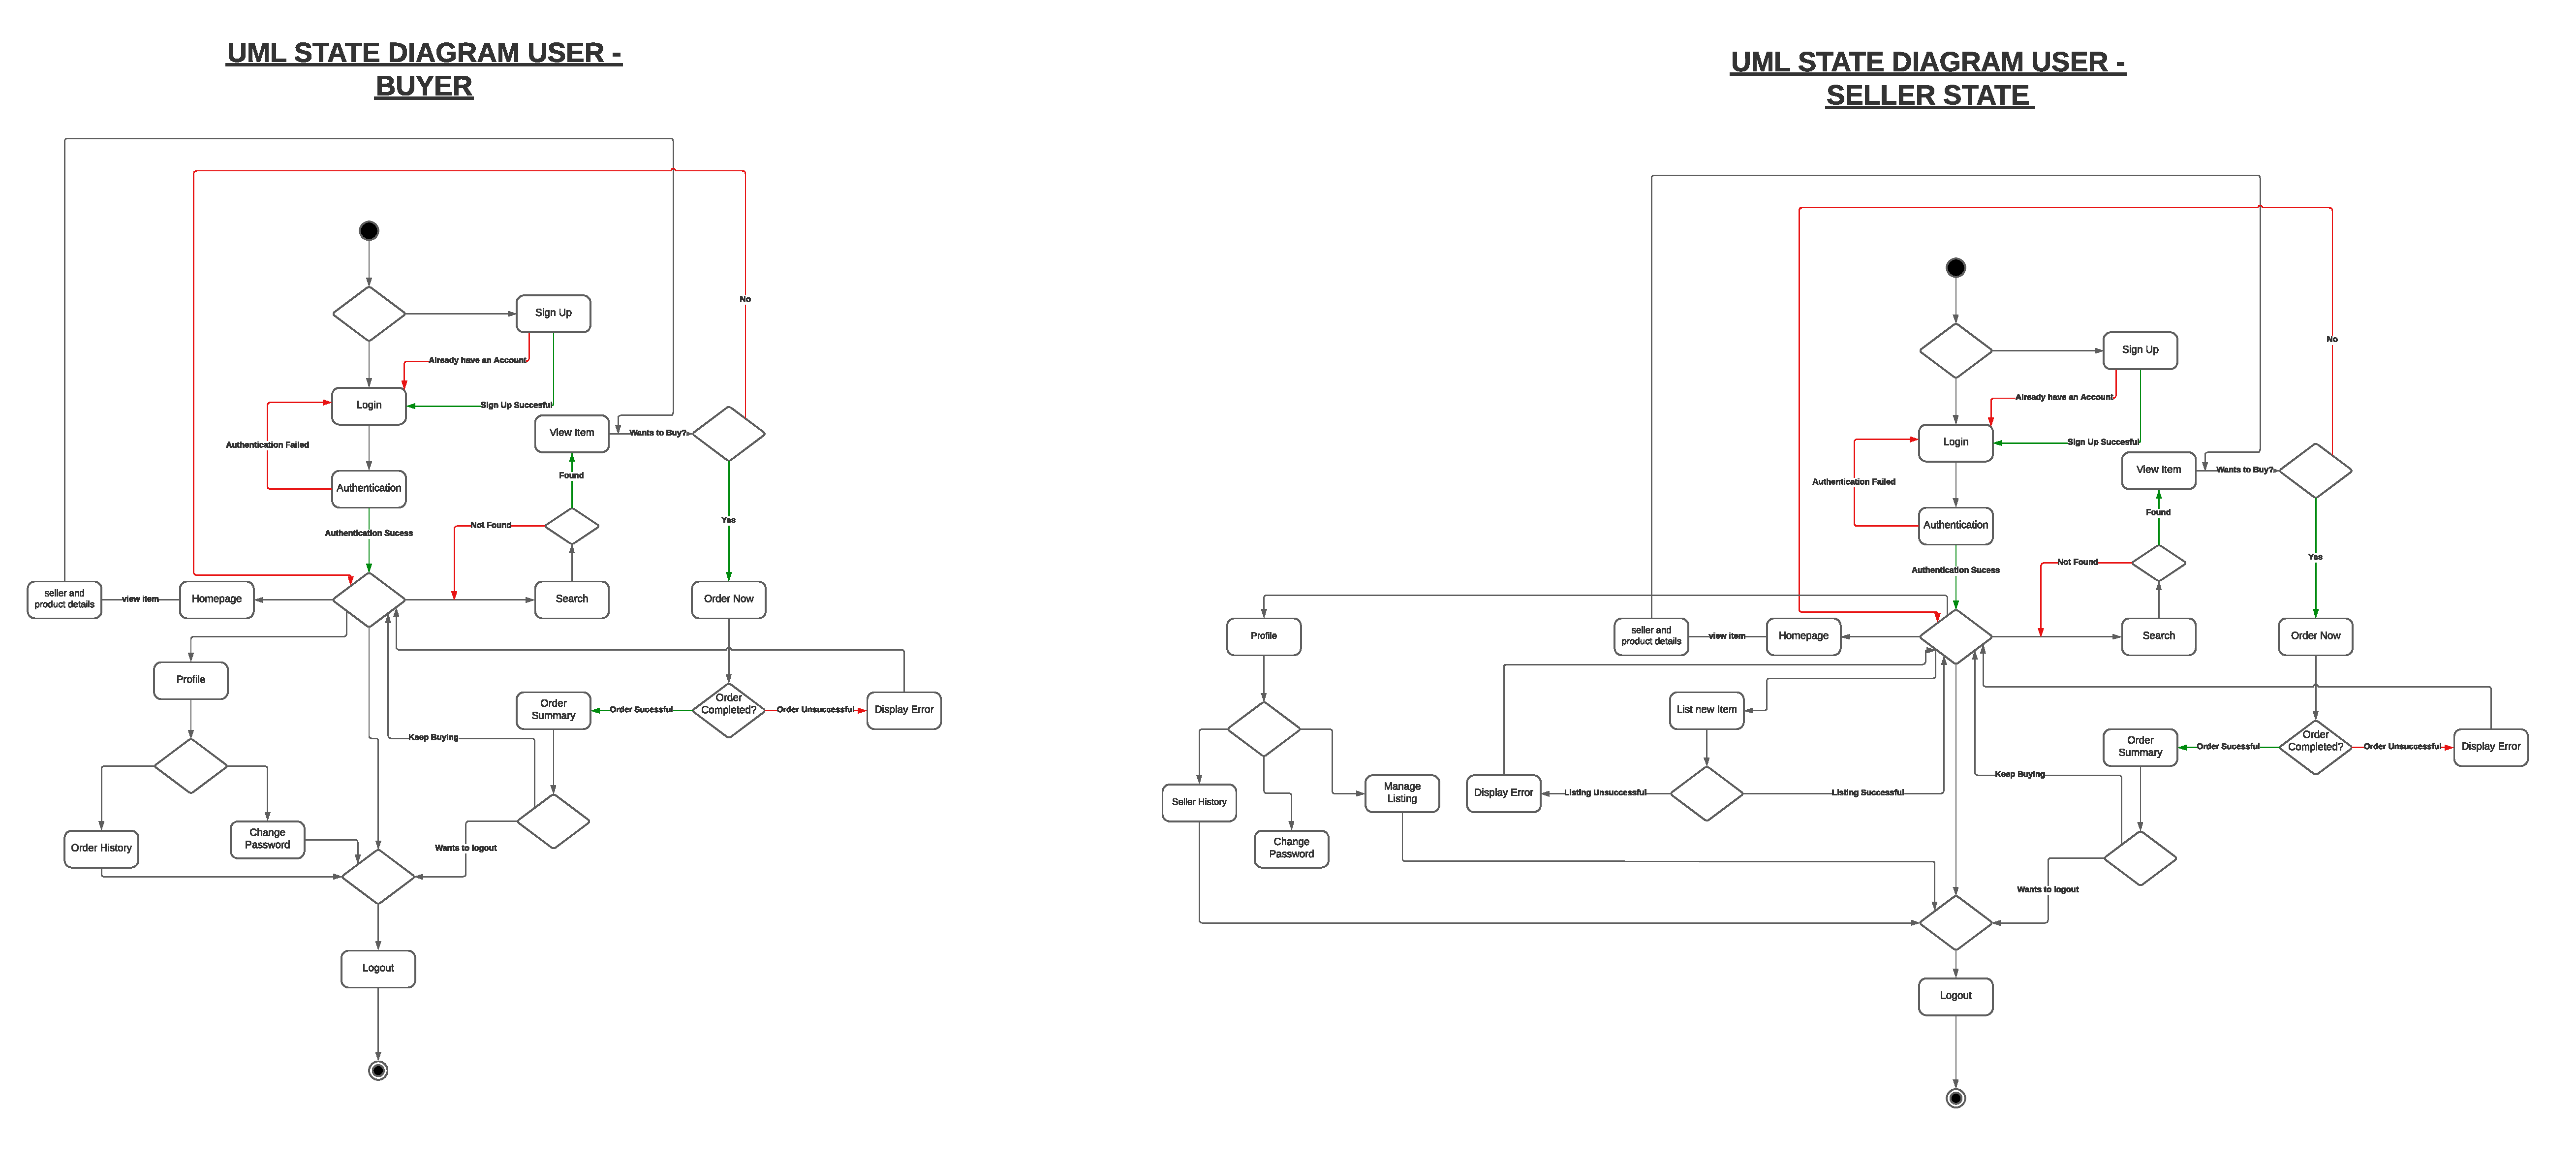
\includepdf[scale=1.0,pages=1]{../Descriptive-Part/Figures/state-diagram.pdf}
\subsection{Sequence Diagrams}
\section{Alloy}
\hlc{green}{The following figures are the allow model representations for the customer and seller relationships for our system in alloy:}
\createfigure{../Descriptive-Part/Figures/sellerRelationships.png}{Alloy model for a seller}
To model the a seller in our domain model, we followed the domain requirements on what entails being a seller on a typical e-commerce website. Those being:
\begin{itemize}
  \item Username
  \item Password
  \item Email address
  \item A Business license
  \item A business address
  \item A set of shoe entries: that have include information such as:
  \begin{itemize}
    \item Date added
    \item A set of pictures of the product
    \item The physical item to be sold
    \item Video evidence of its review.
  \end{itemize}
\end{itemize}
\createfigure{../Descriptive-Part/Figures/customerRelationships.png}{Alloy model for a customer}
Subsequently, a user (i.e customer) is a minimized version of a seller with fewer signatures attached to them. These were also taken from the domain requirements for what it entails to be a customer in a typical e-commerce website:
\begin{itemize}
  \item Username
  \item Email address
  \item Password
\end{itemize}
\section{Implementation}
\subsection{ER Concept Analysis Diagram}
\hspace{1cm} The ER diagram for the sneakers shopping system consist of tables such as customer, Shoes, Order,
OrderHas, Brand, Model, Cart and Wishlist. The relationship and schema should allow for efficient
querying and retrieval of data. When implementing the system, it will be important to ensure that the
database design aligns with the ER diagram to ensure proper storage. The system will communicate with
the database to display and store information on the platform.
\createfigure{../Analytic-Part/Figures/ER Diagram.jpg}{ER Diagram - Sneaker Shopping System}
\subsection{Home Page}
\hlc{green}{Here is the homepage of the out web app. It shows the eight most recent entries in the database (currently it shows royalty free pictures for testing), along with a navigation bar containing a log in and sign up buttons, along with a search bar with a select menu to search using name model and most recent criteria (currently not connected to backend). At the bottom it shows a test footer.}
\createfigure{../Descriptive-Part/Figures/base-home-page.png}{Base Home Page}
\subsection{Login Portal}
\hlc{green}{This page is a form that allows a customer to log in using a email and password. On a successful login it redirects to the home page displaying a green banner at the top indicating to the customer that they were logged in successfully. On a unsuccessful login the page reloads and displays a red banner on top indicating to the customer that the login attempt was unsuccessful.}
\createfigure{../Descriptive-Part/Figures/successful-login.png}{Login Portal On Successful Login}
\createfigure{../Descriptive-Part/Figures/failed-login.png}{Login Portal On Unsuccessful Login}
\subsection{Sign Up Portal}
\hlc{green}{This page is another form that allows a customer to sign up using a customername, email and password. On a successful sign up, the customer is redirected to the home page, otherwise the sign up page is reloaded along with a banner alert on top with an appropriate error message.}
\createfigure{../Descriptive-Part/Figures/successful-sign-up.png}{Sign Up Portal On Successful Login}
\createfigure{../Descriptive-Part/Figures/failed-sign-up.png}{Sign Up Portal On Unsuccessful Login}
